\documentclass[17pt]{article}

\usepackage[margin=1in, paperwidth=8.5in, paperheight=11in]{geometry}
\usepackage{amsmath}
\usepackage[document]{ragged2e}
\usepackage{graphicx}
\usepackage{listings}
\usepackage{color}
\usepackage[none]{hyphenat}

\definecolor{dkgreen}{rgb}{0,0.6,0}
\definecolor{gray}{rgb}{0.5,0.5,0.5}
\definecolor{mauve}{rgb}{0.58,0,0.82}

\lstset{frame=tb,
  language=Python,
  aboveskip=3mm,
  belowskip=3mm,
  showstringspaces=false,
  columns=flexible,
  basicstyle={\small\ttfamily},
  numbers=none,
  numberstyle=\tiny\color{gray},
  keywordstyle=\color{blue},
  commentstyle=\color{dkgreen},
  stringstyle=\color{mauve},
  breaklines=true,
  breakatwhitespace=true,
  tabsize=3
}

\begin{document}

\title{{Generalized linear model: Bioassay with Stan}}
\maketitle


The Stan model is defined as:

\begin{lstlisting}
data {
    int animals[4];
    int deaths[4];
    vector[4] doses;
    vector[2] mean_val;
    matrix[2, 2] covariance;
    
}

parameters {
    vector[2] alpha_beta;
}

model {
    alpha_beta ~ multi_normal(mean_val, covariance);
    deaths ~ binomial_logit(animals, alpha_beta[1] + alpha_beta[2] * doses);
}
\end{lstlisting}

The $\hat{R}$ values for $\alpha$ and $\beta$ are 1.002 and 1.003 accordingly.

Since $\hat{R}$ values are close to 1, we can say that the model \textbf{has converged}.
\\~\\
Stan also provides a summary of the results. \\
Below is the summary of the experiment.
\begin{center}
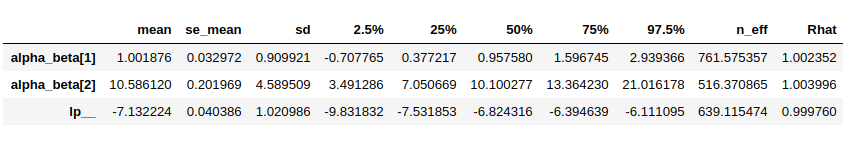
\includegraphics[width=19cm, height=5cm]{summary.png}
\end{center}
\newpage
Below is the scatterplot of the draws.
\begin{center}
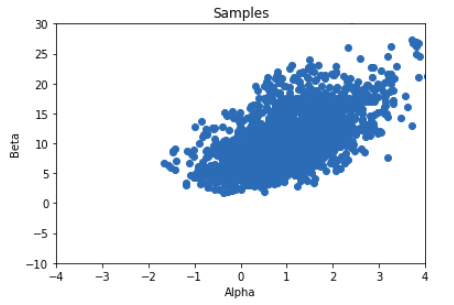
\includegraphics[width=10cm, height=5cm]{samples.png}
\end{center}

Stan also provides useful visualizations.

Below is a visualization of $\alpha$ and $\beta$ provided by Stan.
\begin{center}
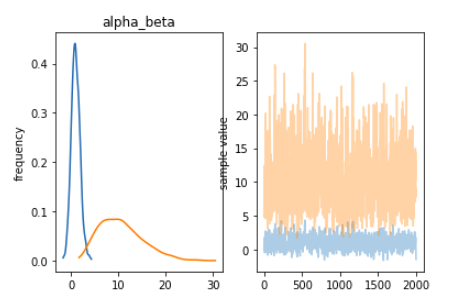
\includegraphics[width=10cm, height=5cm]{alpha_beta.png}
\end{center}


\newpage

\begin{align}
\textbf{SOURCE CODE}
\end{align}

\begin{lstlisting}
import pystan
import numpy as np
import pandas as pd
import matplotlib.pyplot as plt

corr = 0.5
sigma_alpha = 2
sigma_beta = 10
mu_alpha = 0
mu_beta = 10

animals = np.array([5, 5, 5, 5])
doses = np.array([-0.86, -0.30, -0.05, 0.73])
deaths = np.array([0, 1, 3, 5])

mean = np.array([mu_alpha, mu_beta])
covariance = np.array([[sigma_alpha ** 2, corr * sigma_alpha * sigma_beta],
                       [corr * sigma_alpha * sigma_beta, sigma_beta**2]])
                       

bioassay_code = """
data {
    int animals[4];
    int deaths[4];
    vector[4] doses;
    vector[2] mean_val;
    matrix[2, 2] covariance;
    
}

parameters {
    vector[2] alpha_beta;
}

model {
    alpha_beta ~ multi_normal(mean_val, covariance);
    deaths ~ binomial_logit(animals, alpha_beta[1] + alpha_beta[2] * doses);
}
"""

bioassay_dat = {'animals': animals,
                'doses': doses,
                'deaths': deaths,
                'mean_val': mean,
                'covariance': covariance
               }

sm = pystan.StanModel(model_code = bioassay_code)
fit = sm.sampling(data = bioassay_dat, iter=1000, chains=4)


summary = fit.summary()
summary = pd.DataFrame(summary['summary'], columns=summary['summary_colnames'], index=summary['summary_rownames'])
alpha_rhat = summary['Rhat'][0]
beta_rhat = summary['Rhat'][1]
print('The Rhat values are: {0} {1}'.format(alpha_rhat, beta_rhat))

alpha_beta = fit.extract(permuted=True)['alpha_beta']
alpha = alpha_beta[:,0]
beta = alpha_beta[:,1]

fit.plot()
summary


# Plot the data
plt.scatter(alpha, beta)
plt.xlim(-4, 4)
plt.ylim(-10, 30)
plt.xlabel('Alpha')
plt.ylabel('Beta')
plt.title('Samples')
plt.show()                       
\end{lstlisting}


\end{document}